\documentclass{ximera}
 

\usepackage{epsfig}

\graphicspath{
  {./}
  {figures/}
}

\usepackage{morewrites}
\makeatletter
\newcommand\subfile[1]{%
\renewcommand{\input}[1]{}%
\begingroup\skip@preamble\otherinput{#1}\endgroup\par\vspace{\topsep}
\let\input\otherinput}
\makeatother

\newcommand{\includeexercises}{\directlua{dofile("/home/jim/linearAlgebra/laode/exercises.lua")}}

%\newcounter{ccounter}
%\setcounter{ccounter}{1}
%\newcommand{\Chapter}[1]{\setcounter{chapter}{\arabic{ccounter}}\chapter{#1}\addtocounter{ccounter}{1}}

%\newcommand{\section}[1]{\section{#1}\setcounter{thm}{0}\setcounter{equation}{0}}

%\renewcommand{\theequation}{\arabic{chapter}.\arabic{section}.\arabic{equation}}
%\renewcommand{\thefigure}{\arabic{chapter}.\arabic{figure}}
%\renewcommand{\thetable}{\arabic{chapter}.\arabic{table}}

%\newcommand{\Sec}[2]{\section{#1}\markright{\arabic{ccounter}.\arabic{section}.#2}\setcounter{equation}{0}\setcounter{thm}{0}\setcounter{figure}{0}}

\newcommand{\Sec}[2]{\section{#1}}

\setcounter{secnumdepth}{2}
%\setcounter{secnumdepth}{1} 

%\newcounter{THM}
%\renewcommand{\theTHM}{\arabic{chapter}.\arabic{section}}

\newcommand{\trademark}{{R\!\!\!\!\!\bigcirc}}
%\newtheorem{exercise}{}

\newcommand{\dfield}{{\sf dfield9}}
\newcommand{\pplane}{{\sf pplane9}}

\newcommand{\EXER}{\section*{Exercises}}%\vspace*{0.2in}\hrule\small\setcounter{exercise}{0}}
\newcommand{\CEXER}{}%\vspace{0.08in}\begin{center}Computer Exercises\end{center}}
\newcommand{\TEXER}{} %\vspace{0.08in}\begin{center}Hand Exercises\end{center}}
\newcommand{\AEXER}{} %\vspace{0.08in}\begin{center}Hand Exercises\end{center}}

% BADBAD: \newcommand{\Bbb}{\bf}

\newcommand{\R}{\mbox{$\Bbb{R}$}}
\newcommand{\C}{\mbox{$\Bbb{C}$}}
\newcommand{\Z}{\mbox{$\Bbb{Z}$}}
\newcommand{\N}{\mbox{$\Bbb{N}$}}
\newcommand{\D}{\mbox{{\bf D}}}
\usepackage{amssymb}
%\newcommand{\qed}{\hfill\mbox{\raggedright$\square$} \vspace{1ex}}
%\newcommand{\proof}{\noindent {\bf Proof:} \hspace{0.1in}}

\newcommand{\setmin}{\;\mbox{--}\;}
\newcommand{\Matlab}{{M\small{AT\-LAB}} }
\newcommand{\Matlabp}{{M\small{AT\-LAB}}}
\newcommand{\computer}{\Matlab Instructions}
\newcommand{\half}{\mbox{$\frac{1}{2}$}}
\newcommand{\compose}{\raisebox{.15ex}{\mbox{{\scriptsize$\circ$}}}}
\newcommand{\AND}{\quad\mbox{and}\quad}
\newcommand{\vect}[2]{\left(\begin{array}{c} #1_1 \\ \vdots \\
 #1_{#2}\end{array}\right)}
\newcommand{\mattwo}[4]{\left(\begin{array}{rr} #1 & #2\\ #3
&#4\end{array}\right)}
\newcommand{\mattwoc}[4]{\left(\begin{array}{cc} #1 & #2\\ #3
&#4\end{array}\right)}
\newcommand{\vectwo}[2]{\left(\begin{array}{r} #1 \\ #2\end{array}\right)}
\newcommand{\vectwoc}[2]{\left(\begin{array}{c} #1 \\ #2\end{array}\right)}

\newcommand{\ignore}[1]{}


\newcommand{\inv}{^{-1}}
\newcommand{\CC}{{\cal C}}
\newcommand{\CCone}{\CC^1}
\newcommand{\Span}{{\rm span}}
\newcommand{\rank}{{\rm rank}}
\newcommand{\trace}{{\rm tr}}
\newcommand{\RE}{{\rm Re}}
\newcommand{\IM}{{\rm Im}}
\newcommand{\nulls}{{\rm null\;space}}

\newcommand{\dps}{\displaystyle}
\newcommand{\arraystart}{\renewcommand{\arraystretch}{1.8}}
\newcommand{\arrayfinish}{\renewcommand{\arraystretch}{1.2}}
\newcommand{\Start}[1]{\vspace{0.08in}\noindent {\bf Section~\ref{#1}}}
\newcommand{\exer}[1]{\noindent {\bf \ref{#1}}}
\newcommand{\ans}{}
\newcommand{\matthree}[9]{\left(\begin{array}{rrr} #1 & #2 & #3 \\ #4 & #5 & #6
\\ #7 & #8 & #9\end{array}\right)}
\newcommand{\cvectwo}[2]{\left(\begin{array}{c} #1 \\ #2\end{array}\right)}
\newcommand{\cmatthree}[9]{\left(\begin{array}{ccc} #1 & #2 & #3 \\ #4 & #5 &
#6 \\ #7 & #8 & #9\end{array}\right)}
\newcommand{\vecthree}[3]{\left(\begin{array}{r} #1 \\ #2 \\
#3\end{array}\right)}
\newcommand{\cvecthree}[3]{\left(\begin{array}{c} #1 \\ #2 \\
#3\end{array}\right)}
\newcommand{\cmattwo}[4]{\left(\begin{array}{cc} #1 & #2\\ #3
&#4\end{array}\right)}

\newcommand{\Matrix}[1]{\ensuremath{\left(\begin{array}{rrrrrrrrrrrrrrrrrr} #1 \end{array}\right)}}

\newcommand{\Matrixc}[1]{\ensuremath{\left(\begin{array}{cccccccccccc} #1 \end{array}\right)}}



\renewcommand{\labelenumi}{\theenumi)}
\newenvironment{enumeratea}%
{\begingroup
 \renewcommand{\theenumi}{\alph{enumi}}
 \renewcommand{\labelenumi}{(\theenumi)}
 \begin{enumerate}}
 {\end{enumerate}\endgroup}



\newcounter{help}
\renewcommand{\thehelp}{\thesection.\arabic{equation}}

%\newenvironment{equation*}%
%{\renewcommand\endequation{\eqno (\theequation)* $$}%
%   \begin{equation}}%
%   {\end{equation}\renewcommand\endequation{\eqno \@eqnnum
%$$\global\@ignoretrue}}

%\input{psfig.tex}

\author{Martin Golubitsky and Michael Dellnitz}

%\newenvironment{matlabEquation}%
%{\renewcommand\endequation{\eqno (\theequation*) $$}%
%   \begin{equation}}%
%   {\end{equation}\renewcommand\endequation{\eqno \@eqnnum
% $$\global\@ignoretrue}}

\newcommand{\soln}{\textbf{Solution:} }
\newcommand{\exercap}[1]{\centerline{Figure~\ref{#1}}}
\newcommand{\exercaptwo}[1]{\centerline{Figure~\ref{#1}a\hspace{2.1in}
Figure~\ref{#1}b}}
\newcommand{\exercapthree}[1]{\centerline{Figure~\ref{#1}a\hspace{1.2in}
Figure~\ref{#1}b\hspace{1.2in}Figure~\ref{#1}c}}
\newcommand{\para}{\hspace{0.4in}}

\renewenvironment{solution}{\suppress}{\endsuppress}

\ifxake
\newenvironment{matlabEquation}{\begin{equation}}{\end{equation}}
\else
\newenvironment{matlabEquation}%
{\let\oldtheequation\theequation\renewcommand{\theequation}{\oldtheequation*}\begin{equation}}%
  {\end{equation}\let\theequation\oldtheequation}
\fi

\makeatother

\begin{document}
\begin{computerExercise} \label{c9.1.8}
Foxes (the predators) and rabbits (the prey) coexist in an isolated area.
In equilibrium, there are 200 foxes and 10,000 rabbits.  When isolated from
the foxes, the rabbit population doubles every year.  When isolated from 
the rabbits, the fox population decreases at the rate of 10\% per year. 
Supposing that the fox-rabbit populations are modeled by the predator-prey
equations \eqref{e:PP}, answer the following questions.
\begin{itemize}
\item[(a)]  	What are the values of $\mu_1,\mu_2,\sigma_1,\sigma_2$ in 
\eqref{e:PP}.
\item[(b)]	After a storm 1,200 rabbits and 110 foxes remain in the area.
According to this model, what will the fox population be after three years?  
{\bf Hint:}  Use the {\sf Specify a computation interval} on the 
{\sf \PPLANE Keyboard input} menu.
\item[(c)]	After the storm, what is the maximum number of rabbits that 
this model predicts will inhabit the area.
\item[(d)]	How many years will it take the rabbit population to reach 
this maximum number for the first time?
\end{itemize}

\begin{solution}

\ans (a) $\mu_1=\ln(2)$, $\mu_2=\ln(0.9)$, $\sigma_1 = -\frac{\ln(2)}{200}$,
and $\sigma_2 = -\frac{\ln(0.9)}{10000}$; (b) $86$ foxes; (c) 48,000 rabbits; 
(d) $10.5$ years.

\soln In the predator-prey equations $x$ denotes the prey population --- 
the rabbits --- and $y$ denotes the predator population --- the foxes.

\noindent (a) When $y=0$, the $\dot{x}$ equation can be solved for 
$x(t)=e^{\mu_1t}x_0$.  Thus when there are no foxes, the rabbit population 
doubles each year if $e^{\mu_1}=2$, that is, $\mu_1=\ln(2)$.  Similarly, when
$x=0$ the $\dot{y}$ equation can be solved for $y(t)=e^{\mu_2 t}y_0$.  So the
fox population decreases by 10\% each year in the absence of rabbits if 
$e^{\mu_2}=0.9$, that is, $\mu_2=\ln(0.9)$.

Next observe that there is just one equilibrium $(x_1,y_1)$ for the 
predator-prey equations when both populations are nonzero and that 
equilibrium is 
\[
(x_1,y_1) = \left(-\frac{\mu_2}{\sigma_2},-\frac{\mu_1}{\sigma_1}\right) = 
\left(-\frac{\ln(0.9)}{\sigma_2},-\frac{\ln(2)}{\sigma_1}\right) = 
(10000,200).
\]
So
\[
\sigma_1 = -\frac{\ln(2)}{200}<0 \quad \mbox{and} \quad
\sigma_2 = -\frac{\ln(0.9)}{10000}>0.
\]
Thus, under these conditions, the predator-prey model is:
\begin{equation}  \label{E:PPspec}
\begin{array}{rcl}
\dot{x} & = & x(\ln(2) - \ln(0.9)y/10000) \\
\dot{y} & = & y(\ln(0.9) - \ln(2)x/200),
\end{array}
\end{equation}

\noindent (b) Using the {\sf Keyboard input} button and the {\sf Specify a
computation interval} in that menu, we can compute the solution with initial
condition $(x_0,y_0)=(1200,110)$ until time $t=3$ years.  The result is that
the number of foxes is $86$ as can be seen from the time series in 
Figure~\ref{c9.1.8}a.

\noindent (c)  Using the {\sf Keyboard input} button, we can start
integrating the differential equation with initial condition
$(x_0,y_0)=(1200,110)$.  Graphing the $x$ time series (the rabbit population)
we get the result shown in Figure~\ref{c9.1.8}b.  Specifically, the 
maximum is approximately 48,000 rabbits. 

\noindent (d)  The maximum rabbit population occurs for the first time about 
$10.5$ years after the storm.

\begin{figure}[htb]
     \centerline{%
     \psfig{file=exfigure/PPinit2.eps,width=2.75in}
     \psfig{file=exfigure/PPinit.eps,width=2.75in}}
     \caption{(Left) Time series $y$ vs. $t$ of (\protect\ref{E:PPspec}) 
	showing population of foxes after three years. (Right) Time series $x$ 
	vs. $t$ of (\protect\ref{E:PPspec}) showing maximum rabbit population.}
     \exercaptwo{c9.1.8}
\end{figure}


\end{solution}
\end{computerExercise}
\end{document}
